%priprava posamezne ure
%tukaj zaporedoma napisemo{st. zaporedne ure}{datum}{naslov}{poglavje}{oblika dela}{pripomocki}
\begin{priprava}{}{}{Verjetnostni račun}{Uvod}{frontalna}{tabla}

Motivacija: Kolikšna je verjetnost, da pri metu kocke pade 6?

\textbf{Pojmi:} \didopomba{na primeru meta kocke}

POSKUS: vsako dejanje, ki se dogaja v določenih pogojih (met kocke/kovanca, vlečenje kroglic iz posode, žreb \ldots)

DOGODEK: kar se zgodi (označujemo s velikimi tiskanimi črkami: A, B, C, D \ldots)
\begin{itemize}
    \item GOTOV DOGODEK: dogodek, ki se zagotovo zgodi (pri metu kocke pade manj kot 7)
    \item NEMOGOČ DOGODEK: dogodek, ki se ne more zgoditi (pade 9 pik)
    \item SLUČAJNI DOGODEK: dogodek, ki se včasih zgodi, včasih pa ne (padejo 4 pike)
\end{itemize}

\textcolor{red}{\textbf{Verjetnost} je število -- razmerje med ugodnimi izidi in vsemi izidi:}
$$ P(A) = \frac{\text{št. ugodnih izidov}}{\text{št. vseh izidov}} $$

\didopomba{Najprej nekaj enostavnih vaj, kjer lahko preštevamo dogodke. Naj na začetku povejo za vsak primer -- kaj je dogodek, kaj je uspeli poskus, kaj so vsi poskusi.}

\vaje{
Vaje:
\begin{itemize}
    \item \didopomba{uvodni primer} Mečemo eno kocko. Kolikšna je verjetnost, da pade 6? Da pade manj kot 5? Da pade soda številka?
    \item Mečemo dve kocki. Kolikšna je verjetnost, da na eni kocki pade 1? Da je na obeh liho število? Da je padeta 4 in 6? \didopomba{za prvič lahko narediš 6x6 tabelico vseh možnih parov in se ven prešteje pare}
    \item Desetkrat vržemo kovanec. Kolikšna je verjetnost, da vsakič pade grb? Kaj pa, da pade cifra trikrat?
\end{itemize}
}


Z dogodki računamo podobno kot z množicami. \didopomba{slikce zraven vsake vrste + praktični primeri!}

\begin{itemize}
    \item \emph{Vsota dogodkov $ A $ in $ B $}: dogodek, ki se zgodi takrat, ko se zgodi dogodek $ A $ ali $ B $ ali oba hkrati. \didopomba{npr. pade 3 ali liho število}
    \item \emph{Produkt dogodkov $ A $ in $ B $}: dogodek, ki se zgodi, ko se zgodita oba dogodka $ A $ in $ B $ hkrati. \didopomba{pade liho število, manjše od štiri}
    \item \emph{Nasprotni dogodek (komplement) dogodka $ A $}: dogodek, ki se zgodi, ko se \emph{ne} zgodi dogodek $ A $. \didopomba{njuna unija pa je gotov dogodek; npr. ne pade 4}
    \item \emph{Razlika dogodkov $ A $ in $ B $}: dogodek, ki se zgodi, ko se zgodi $ A $, vendar se hkrati \emph{ne} zgodi $ B $. \didopomba{pade liho število, ki ni deljivo s 3}
    \item \emph{Poddogodek $ A $ dogodka $ B $}: Če se zgodi $ B $, se zgodi tudi $ A $, obratno pa ni nujno res. \didopomba{primer?}
\end{itemize}

\newpage

\begin{figure}[h]
    \centering
    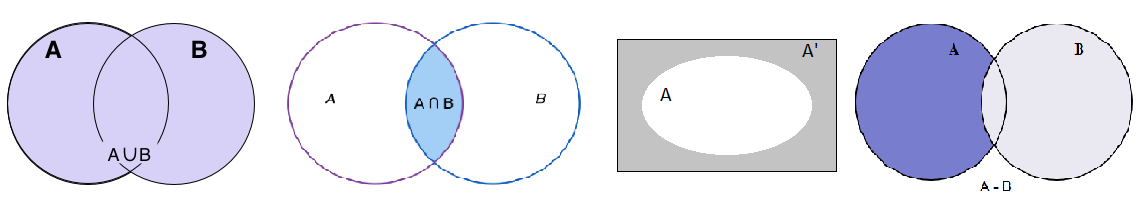
\includegraphics[width=\textwidth]{slike/dogodki.png}
\end{figure}

Aksiomi Kolmogorova: \didopomba{aksiom je trditev, ki jo privzamemo kot veljavno}
\begin{enumerate}
    \item $ P(A) \geq 0 $
    \item $ P(\text{gotov dogodek}) = 1 $
    \item $ P(A \cup B) = P(A) + P(B) $, če sta dogodka \textbf{nezdružljiva} (se ne moreta zgoditi hkrati, npr. v enem metu pade 1 in 3)
\end{enumerate}
Iz teh lastnosti sledi: \didopomba{naj sami ugotavljajo, kaj je po enačaju}
\begin{itemize}
    \item $ P(A \cup A^c) = P(A) + P(A^c) = 1 \rightarrow P(A) = 1 - P(A^c) $
    \item $ P(\text{nemogoč dogodek}) = 0 $ (iz 3., ker sta gotov dogodek in nemogoč dogodek nezdružljiva)
    \item za $ A \subset B $ velja $ P(A) \leq P(B) $ \didopomba{$ B = A \cup (B - A) $, daš čez $ P $ in upoštevaš $ P(B - A) \geq 0 $}
    \item $ P(A \cup B) = P(A) + P(B) - P(A \cap B) $ \didopomba{enako kot pri moči množic}
\end{itemize}
    
\didopomba{Sledi precej vaj (gl. učbenik), ampak še brez produkta in odvisnih dogodkov!}

\end{priprava}